% Imporditud: tools/import_eksperimendid.py
% Allikas: Eesti füüsikaolümpiaadi eksperimendi ülesannete
%   kogu (Rael Kalda, 2023), ülesanne Ü126, lahendus L126.
\setAuthor{EFO žürii}
\setRound{lõppvoor}
\setYear{1996}
\setNumber{G E2}
\setDifficulty{4}
\setTopic{geomeetriline optika}
\setVahendid{luup (koondav 1ääts), millimeetripaber, joonlaud}
\setPunktid{15}
\setAllikas{Eksperimendi kogu Ü126, lahendus lk 99}
\setLahendusseis{toores}

\prob{Luubi suurendus}
$h_2$ $h_1$ f

Luubi suurenduseks S nimetatakse kujutise mõõtme ja eseme vastava mõõtme suhet S = $h_2$/$h_1$. Luubi suurenduse arvutamiseks on käibel valem S = $\rho$/f (1), kus $\rho$ on silma parima nägemise kaugus (25 cm) ja f luubi fookuskaugus. Määrata luubi maksimaalne suurendus millimeetripaberi abil ja võrrelda seda valemi (1) abil arvutatud tulemusega. Kui tulemused erinevad teineteisest oluliselt, püüdke erinevust põhjendada.
\begin{center}
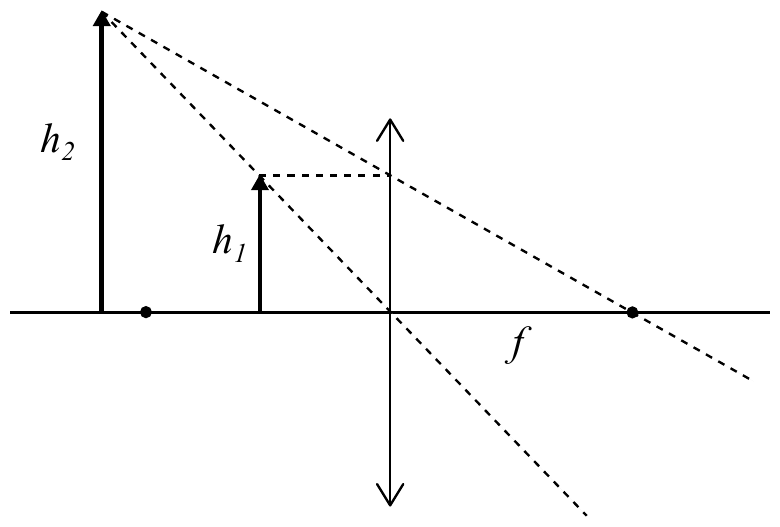
\includegraphics[width=0.55\linewidth]{1996-v3g-ge2-yl.png}
\end{center}

\hint

\solu
Suurenduse määramise idee: võrreldakse läbi luubi paistvate joonte arvu palja silmaga nähtavate joonte arvuga (20\%)

Maksimaalse suurenduse määramine (20\%)

Fookuskauguse määramise idee: $\infty$ tulevate kiirte abil (10\%)

Fookuskauguse määramine (5\%)

Veahinnangud (15\%)

Järeldus: kas tulemused kattuvad vea piires või ei (10\%)

Põhjendus: suurendus oleneb sellest, kui lähedal luup paberile on, sellest oleneb ka kujutise asukoht. See tähendab, et alati ei teki kujutis parima nägemise kaugusele. Silma pingutades võib aga ka neil juhtudel kujutist näha (vms) (20\%)
\probend
